\documentclass[aspectratio=1610]{beamer}

\usetheme{KTH}
\usepackage[utf8]{inputenc}
\usepackage{graphics}
\usepackage{graphicx}
\usepackage{booktabs}
\usepackage{amsmath}
\usepackage{mathtools}
\usepackage[makeroom]{cancel}
\usepackage[utf8]{inputenc}
\usepackage{amssymb}
\usepackage{ragged2e}
\usepackage{lipsum}
\usepackage{tikz}
\usepackage{array}
\usepackage{amsmath,amsfonts,amssymb}
\usepackage[export]{adjustbox}

\usepackage{paralist}

\usefonttheme{serif}


\begin{document}
\begin{frame}[noframenumbering,plain]

  \vspace{0.02\textheight}
  
\begin{columns}[]
\column{37em}
\Large{\centerline{\usebeamercolor[fg]{title}SF1518/19 Mästarprov 13: Strömkretsen}}

\vspace{0.1\textheight}

\small{\centerline{Hassan Al Noori}}
\scriptsize{\centerline{\tt hassanan@kth.se}}
\scriptsize{\centerline{}}
\end{columns}
\end{frame}

%------------------------------------------------
\usebackgroundtemplate{\vbox{\null\vspace{3mm}
  \hspace{3mm}\pgfuseimage{kthlogosmall}\par
  \vspace{72mm}\hbox{\hspace{-75mm}\pgfuseimage{kthplatta}}}}

%------------------------------------------------
\begin{frame}
\frametitle{LC-circuit}
\begin{columns}
\column{37em}
\begin{itemize}
    \item<2-> What is an LC-circuit?
\end{itemize}
\centerline{\hspace*{1cm}\includegraphics[width=8cm]{figs/Stromkrets.png}}


\end{columns}
\end{frame}
%------------------------------------------------
\begin{frame}
\frametitle{RFID}
\begin{columns}
\column{37em}
\hspace*{5cm}\includegraphics[width=5cm]{figs/rfid.png}
\end{columns}
\end{frame}
%------------------------------------------------
\begin{frame}
\frametitle{Electronic article surveillance}
\begin{columns}
\column{37em}
\hspace*{5cm}\includegraphics[width=4cm]{figs/barcode.png}
\end{columns}
\end{frame}
%------------------------------------------------
\begin{frame}
\frametitle{Project statement}
\begin{columns}
\column{37em}
\begin{itemize}\itemsep1em
  \item<2-> What is the current in the circuit?
  \item<3-> How is the current affected by the voltage?
  \item<4-> Prove $E(t)$ is constant
  \item<5-> How big is the error?
  \item<6-> Fourier transform
  \item<7-> Voluntary part
\end{itemize}
\end{columns}
\end{frame}
%------------------------------------------------
\begin{frame}
\frametitle{Mathematical formulation}
\begin{columns}
\column{34em}
\huge
\begin{tabular}{c c}
	{$\!\begin{aligned}
		L = \frac{L_{0}}{1+I^{2}}
	\end{aligned} $}&
		{$\!\begin{aligned}
		U = L\frac{dI}{dt}
	\end{aligned}$}\\\\
		{$\!\begin{aligned}
		I = -C\frac{dU}{dt}
	\end{aligned}$}&
		{$\!\begin{aligned}
		\quad t=0, \quad I=0,\quad \frac{dI}{dt}=\frac{U_{0}}{L_{0}}
	\end{aligned}$}
\end{tabular}
\end{columns}
\end{frame}
%------------------------------------------------
\begin{frame}
\frametitle{Mathematical formulation}
\huge
\begin{align*}
\frac{d^{2}I}{dt^{2}}=\frac{2I}{1+I^{2}}\left(\frac{dI}{dt}\right)^{2}-\frac{I\left(1+I^{2}\right)}{L_{0}C}
\end{align*}
\end{frame}
%------------------------------------------------
\begin{frame}
\frametitle{Mathematical formulation}
\begin{columns}
\column{37em}
\huge
\begin{align*}\\
\tilde{y}'(t) =
\begin{bmatrix}
y_{1}'(t) \\ 
y_{2}'(t) \\
\end{bmatrix}
= \begin{bmatrix}
y_{2}(t)\\
\frac{2y_{1}(t)y_{2}^{2}(t)}{1+y_{1}(t)^2}-\frac{1+y_{1}(t)^{2}}{L_{0}C}\\
\end{bmatrix}
\end{align*}
\end{columns}
\end{frame}
%------------------------------------------------
\begin{frame}
\frametitle{Numerical Methods - Runge Kutta 4}
\begin{columns}
\column{2em}
\Large
  \begin{align*}
  K_{1}&=hf(x_{n},y_{n})\\
  K_{2}&=hf(x_{n}+\frac{h}{2},y_{n}+\frac{k_{1}}{2})\\
  K_{3}&=hf(x_{n}+\frac{h}{2},y_{n}+\frac{k_{2}}{2})\\
  K_{4}&=hf(x_{n}+h,y_{n}+k_{3})\\
  y_{n+1}&=y_{n}+\frac{1}{6}\left(K_{1}+2K_{2}+2K_{3}+K_{4}\right)+O(h^{5})
  \end{align*}
\end{columns}
\end{frame}

%------------------------------------------------
\begin{frame}
\frametitle{Mathematical formulation}
\begin{columns}
\column{37em}
\huge
\begin{align*}
E(t) & = U(t)^{2}-log(1+I(t)^{2})\\
\end{align*}
\end{columns}
\end{frame}
%------------------------------------------------
\begin{frame}
\frametitle{Mathematical formulation}
\begin{columns}
\column{37em}
\huge
\begin{align*}
\frac{dE}{dt} & = \frac{d}{dt}\left(U(t)^{2}-log(1+I(t)^{2})\right)\\
\end{align*}
\end{columns}
\end{frame}
%------------------------------------------------
\begin{frame}
\frametitle{Mathematical formulation}
\begin{columns}
\column{37em}
\huge
\begin{align*}
& = \frac{d}{dt}\left(\left(\frac{L_{0}\frac{dI}{dt}}{1+I(t)^{2}})\right)^{2}-log\left(1+I(t)^{2}\right)\right) \\
\end{align*}
\end{columns}
\end{frame}
%------------------------------------------------
\begin{frame}
\frametitle{Mathematical formulation}
\begin{columns}
\column{37em}
\huge
\begin{align*}
& = \frac{d}{dt}\left(\frac{L_{0}\frac{dI}{dt}}{1+I(t)^{2}}\right)^{2}-\frac{d}{dt}\left(log\left(1+I(t)^{2}\right)\right)\\
\end{align*}
\end{columns}
\end{frame}
%------------------------------------------------
\begin{frame}
\frametitle{Mathematical formulation}
\begin{columns}
\column{37em}
\huge
\begin{align*}
& = ...
\end{align*}
\end{columns}
\end{frame}
%------------------------------------------------
\begin{frame}
\frametitle{Mathematical formulation}
\begin{columns}
\column{37em}
\LARGE
\begin{align*}
& = 2\left({\frac{\frac{dI}{dt}\left(1+I(t)^{2}\left(\frac{d^{2}I}{dt^{2}}\right)-2I(t)\left(\frac{dI}{dt}\right)^{2}\right)}{\left(1+I(t)^{2}\right)^{3}}} -   {\frac{I(t)\left(\frac{dI}{dt}\right)}{\left(1+I(t)^{2}\right)}}\right)\\
\end{align*}
\end{columns}
\end{frame}
%------------------------------------------------
\begin{frame}
\frametitle{Mathematical formulation}
\begin{columns}
\column{37em}
\LARGE
\begin{align*}
& = 2\left(\frac{\frac{dI}{dt}}{1+I(t)^{2}}\right)   \left({\frac{1+I(t)^{2}\left(\frac{d^{2}I}{dt^{2}}\right)-2I(t)\left(\frac{dI}{dt}\right)^{2}}{\left(1+I(t)^{2}\right)^{2}}} -   {\frac{I(t)}{1}}\right)\\
\end{align*}
\end{columns}
\end{frame}
%------------------------------------------------
\begin{frame}
\frametitle{Mathematical formulation}
\begin{columns}
\column{37em}
\large
\begin{align*}
\frac{dE}{dt} & = 0 \quad \forall \quad t \in \mathbb{R} \quad \Longleftrightarrow \frac{d}{dt}I(0) = 0 \quad or \quad I(0)= 0 \quad \because \\
\frac{dE}{dt} &= 0 \Longrightarrow 
{\frac{d^{2}I}{dt^{2}}}=\left(\frac{2I(t)\frac{dI}{dt}}{1+I(t)^{2}}+\frac{4\left(\frac{dI}{dt}\right)^{3}I(t)}{\left(1+I(t)^{2}\right)^{3}}\right)\frac{\left(1+I(t)^{2}\right)^{2}}{2\left(\frac{dI}{dt}\right)}
\end{align*}
Which by definition is a second order autonomous ODE. Thus, If $I=c$ is a specific solution, then its phase line is indenpendent of the time at which initial conditions are applied. Hence
\begin{align*}
\frac{d^{2}I}{dt^{2}}=0,\quad I_{0}=0 \quad \therefore\quad\frac{dE}{dt}=0\\
\square
\end{align*}
\end{columns}
\end{frame}
%------------------------------------------------
\begin{frame}
\frametitle{$U_{0}= 240V$}
\begin{columns}
	\column{0.65\textwidth}
		\begin{figure}		
			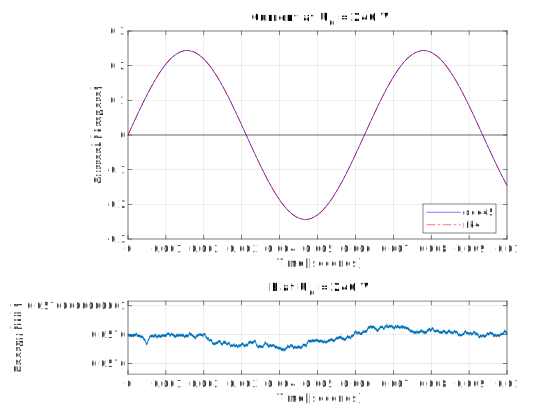
\includegraphics[scale=0.25]{figs/240V + E.png}
      	\end{figure}
	\column{0.55\textwidth}
      	
\end{columns}    
\end{frame}
%------------------------------------------------
\begin{frame}
\frametitle{$U_{0}= 1200V$}
\begin{columns}
		\column{0.65\textwidth}
		\begin{figure}		
			\includegraphics[scale=0.25]{figs/1200V + E.png}
      	\end{figure}
		\column{0.55\textwidth}	
\end{columns} 
\end{frame}
%------------------------------------------------
\begin{frame}
\frametitle{$U_{0}= 2400V$}
\begin{columns}
		\column{0.65\textwidth}
		\begin{figure}		
			\includegraphics[scale=0.25]{figs/2400V + E.png}
      	\end{figure}
		\column{0.55\textwidth}	
\end{columns} 
\end{frame}
%------------------------------------------------
\begin{frame}
\frametitle{Fourier analysis}
\large
\begin{align*}
I(t)=a_{1}sin(\omega t)+a_{2}sin(2\omega t)+a_{3}sin(3\omega t)+\cdots, \quad  \quad \omega = 2\pi/T\\
\end{align*}
\begin{align*}
a_{k} = \frac{2}{T}\int_{0}^{T} I(t)sin(k\omega t)dt,\quad k=1,2,3....
\end{align*}
\end{frame}
%------------------------------------------------

\begin{frame}
\frametitle{Fourier analysis}
\begin{columns}
\column{37em}
\begin{itemize}
	\item<1-> Trapezoidal integration for periodic functions\\
 	 \begin{align*}
	 	 T(h)& = \frac{h}{2}\left(f_{0}+f_{m}+  2\sum_{m-1}^{i=1} y_{i}\right)
 	 \end{align*} 
	 \begin{align*}
	 I &= T(h)-\frac{f'(b)-f'(a)}{12}h^2+\frac{f'''(b)-f'''(a)}{720}h^4-\frac{f^{(5)}(b)-f^{(5)}(a)}{30240}h^6+O(h^8)
			\end{align*}
\end{itemize}

\end{columns}
\end{frame}
%------------------------------------------------
\begin{frame}
\frametitle{$U_{0}= 240V$}
	\begin{columns}
		\column{0.55\textwidth}
			\begin{figure}
				\includegraphics[scale=0.25]{figs/fourier vs rk4 240.png}
			\end{figure}
		\column{0.55\textwidth}
			\begin{figure}
				\includegraphics[scale=0.25]{figs/fourier comparison 240.png}
			\end{figure}
	\end{columns}
\end{frame}
%------------------------------------------------
\begin{frame}
\frametitle{$U_{0}= 1200V$}
	\begin{columns}
		\column{0.55\textwidth}
			\begin{figure}
				\includegraphics[scale=0.25]{figs/fourier vs rk4 1200.png}
			\end{figure}
		\column{0.55\textwidth}
			\begin{figure}
				\includegraphics[scale=0.25]{figs/fourier comparison 1200.png}
			\end{figure}
	\end{columns}
\end{frame}
%------------------------------------------------
\begin{frame}
\frametitle{$U_{0}= 2400V$}
	\begin{columns}
		\column{0.55\textwidth}
			\begin{figure}
				\includegraphics[scale=0.25]{figs/fourier vs rk4 2400.png}
			\end{figure}
		\column{0.55\textwidth}
			\begin{figure}
				\includegraphics[scale=0.25]{figs/fourier comparison 2400.png}
			\end{figure}
	\end{columns}
\end{frame}
%------------------------------------------------
\begin{frame}
\frametitle{Voluntary part 1}
	\begin{align*}
		I_{max}&\coloneqq 10\\
	\end{align*}
\end{frame}
%------------------------------------------------
\begin{frame}
\frametitle{Voluntary part 1}
	\begin{align*}
		I_{max}&\coloneqq 10\\ \\
		I_{\alpha} &= max \left\lbrace \quad I(U^{*}_{0},L_{0}):U_{0}	\in]240,2400[,L_{0}\in \mathbb{R} \quad\right\rbrace\\ \\
	\end{align*}
\end{frame}
%------------------------------------------------
\begin{frame}
\frametitle{Voluntary part 1}
	\begin{align*}
		I_{max}&\coloneqq 10\\ \\
		I_{\alpha} &= max \left\lbrace \quad I(U^{*}_{0},L_{0}):U_{0}	\in]240,2400[,L_{0}\in \mathbb{R} \quad\right\rbrace\\ \\
		g(U^{*}_{0},L_{0})&=0=I_{max}-I_{\alpha}
	\end{align*}
\end{frame}
%------------------------------------------------
\begin{frame}
\frametitle{Voluntary part 1}
	\begin{align*}
		I_{max}&\coloneqq 10\\ \\
		I_{\alpha} &= max \left\lbrace \quad I(U^{*}_{0},L_{0}):U_{0}	\in]240,2400[,L_{0}\in \mathbb{R} \quad\right\rbrace\\ \\
		g(U^{*}_{0},L_{0})&=0=I_{max}-I_{\alpha}
	\end{align*}
\begin{itemize}
	\item<1-> Bisection method
\end{itemize}
\end{frame}
%------------------------------------------------
\begin{frame}
\frametitle{Voluntary part 1}
	\begin{columns}
		\column{0.6\textwidth}
			\begin{figure}
				\includegraphics[scale=0.25]{figs/voluntary_1_Umax.png}
			\end{figure}
		\column{0.6\textwidth}
			\begin{figure}
				\includegraphics[scale=0.25]{figs/voluntary_1_r.png}
			\end{figure}
	\end{columns}
\end{frame}
%------------------------------------------------
\begin{frame}
\frametitle{Voluntary part 2}
	\begin{columns}
		\column{1\textwidth}
		\huge
\begin{align*}
U =L\frac{dI}{dt}\quad\quad
I =-C\frac{dU}{dt}\quad\quad
L = \frac{L_{0}}{1+I^{2}}
\end{align*}
	\end{columns}
\end{frame}
%------------------------------------------------
\begin{frame}
\frametitle{Voluntary part 2}
	\begin{columns}
		\column{1\textwidth}
		\Huge
\begin{align*}
\tilde{y}'=
\begin{bmatrix}
\frac{dI}{dt}\\ \\ 
\frac{dU}{dt}\\
\end{bmatrix}
= \begin{bmatrix}
\frac{1+I^{2}}{L_{0}}{U}\\\\
\frac{\left(\frac{dI}{dt}\right)}{-C}\\
\end{bmatrix}
\end{align*}
	\end{columns}
\end{frame}
%------------------------------------------------
\begin{frame}
\frametitle{Voluntary part 2}
	\begin{columns}
		\column{1\textwidth}
			\begin{figure}
				\includegraphics[scale=0.27]{figs/voluntary_2_240V.png}
			\end{figure}
	\end{columns}
\end{frame}
%------------------------------------------------
\begin{frame}
\frametitle{Voluntary part 2}
	\begin{columns}
		\column{1\textwidth}
			\begin{figure}
				\includegraphics[scale=0.27]{figs/voluntary_2_1200.png}
			\end{figure}
	\end{columns}
\end{frame}
%------------------------------------------------
\begin{frame}
\frametitle{Voluntary part 2}
	\begin{columns}
		\column{1\textwidth}
			\begin{figure}
				\includegraphics[scale=0.27]{figs/voluntary_2_2400V.png}
			\end{figure}
	\end{columns}
\end{frame}
%------------------------------------------------

\begin{frame}
\Large{\centerline{\usebeamercolor[fg]{title}Thanks}}

\vspace{0.25\textheight}

\small{{github - haaln}}\\ \*

\small{{mail - \tt hassanan@kth.se}}
\end{frame}
\end{document}
